\section{Introduction}

\subsection{La question}
Une fenêtre est une suite de cent événements de carnet : ajouts, mises à jour et suppressions d'ordres, avec l'état des meilleures limites après chaque événement. Le challenge CFM demande de dire de quel titre elle provient. La difficulté n'est pas seulement de classer : il faut le faire \emph{dans une autre période}. Le test n'a pas été tiré au hasard parmi les fenêtres du train. Il provient d'autres jours, où les prix, la liquidité affichée, la répartition des volumes entre places de cotation et la taille des ordres ont pu changer.

Un bon classifieur doit donc reconnaître ce qui fait la \emph{signature} d'un titre : sa grille de prix (le tick), ses conventions de quantité (les lots), la façon dont ses ordres vivent et meurent. Il doit le faire sans s'appuyer sur ce qui ne caractérise qu'un \emph{régime} passager, comme une profondeur particulière à une période donnée.

\subsection{Ce qui a changé, en une page}
Le point de départ est le pipeline d'octobre 2025 : un Transformer--BiLSTM qui atteignait \textbf{0,869 en validation} mais seulement \textbf{environ 0,50 au test}. Cet écart, plus que le niveau du modèle, était le vrai problème, et la section~\ref{sec:diagnostic} en dissèque les causes. Le tableau~\ref{tab:resume} résume les différences, et la section~\ref{sec:avantapres} les détaille avec deux schémas complets.

\begin{table}[H]
\centering\small
\begin{tabularx}{\linewidth}{>{\raggedright\arraybackslash}p{2.7cm}>{\raggedright\arraybackslash}X>{\raggedright\arraybackslash}X}
\toprule
& \textbf{Avant} (pipeline d'octobre 2025) & \textbf{Maintenant} (Signature Lab)\\
\midrule
Unités & Spread en unités de prix brutes, spread relatif, momentum, volatilité : des grandeurs de \emph{régime} & \new{Ticks} pour les prix, \new{lots} pour les quantités : des entiers, communs à toutes les fenêtres d'un titre\\
Événement & 16 colonnes : 4 catégories en embeddings, 11 réels normalisés sur le train & \new{11 tokens discrets} (seuils fixés a priori) + 11 canaux continus\\
Ordres & \code{order\_id} utilisé comme un nombre, encodé par un sinus & Rang de première apparition, occurrence, action précédente \emph{du même ordre}, première action ; relation « même ordre » dans l'attention\\
Encodeur & Transformer (2 couches) puis BiLSTM 256 avec attention, $\approx$ 0,8\,M paramètres & Convolutions dilatées + attention relationnelle + pooling attention/moyenne/max\\
Features de fenêtre & Aucune ; filtrage des fenêtres à plus de 10 écarts-types & 11 blocs nommés, cachés et versionnés ($\sim$200 colonnes), passés par un \new{entonnoir de screening}\\
Stress & Aucune partition imitant le test & Queue orientée \new{vers le test} (basse), choix consigné\\
Sélection & \old{Validation aléatoire} 90\,/\,10, arrêt anticipé dessus & Stress équilibré ; la validation aléatoire est jugée non prédictive (écart de 28 points)\\
Sortie & Fusion de modèles (moyennes, maximums) ; pseudo-labels au seuil 0,9 & Moyenne de modèles, \new{équilibrage de Sinkhorn}, \new{vote entre voisins} (transductifs)\\
Période test & Ignorée & \new{Auto-apprentissage} : élèves réentraînés sur les fenêtres test pseudo-étiquetées, deux tours\\
\midrule
Validation \textrightarrow{} LB & $\mathbf{0{,}869}$ \textrightarrow{} $\approx0{,}50$ : l'écart est le vrai problème & $\approx0{,}8$ (par grappes, stress équilibré) \textrightarrow{} $0{,}68$ : un écart mesuré, et chaque gain contrôlé au LB\\
Score public & $\approx0{,}50$ (meilleur score antérieur : $0{,}5072$) & $0{,}5700$ (brut), $0{,}5958$ (équilibré), $0{,}6351$ (V3, voisins), $0{,}6551$ (V4), $\mathbf{0{,}6835}$ (V5)\\
\bottomrule
\end{tabularx}
\caption{Les différences essentielles.}\label{tab:resume}
\end{table}

\begin{figure}[H]
\centering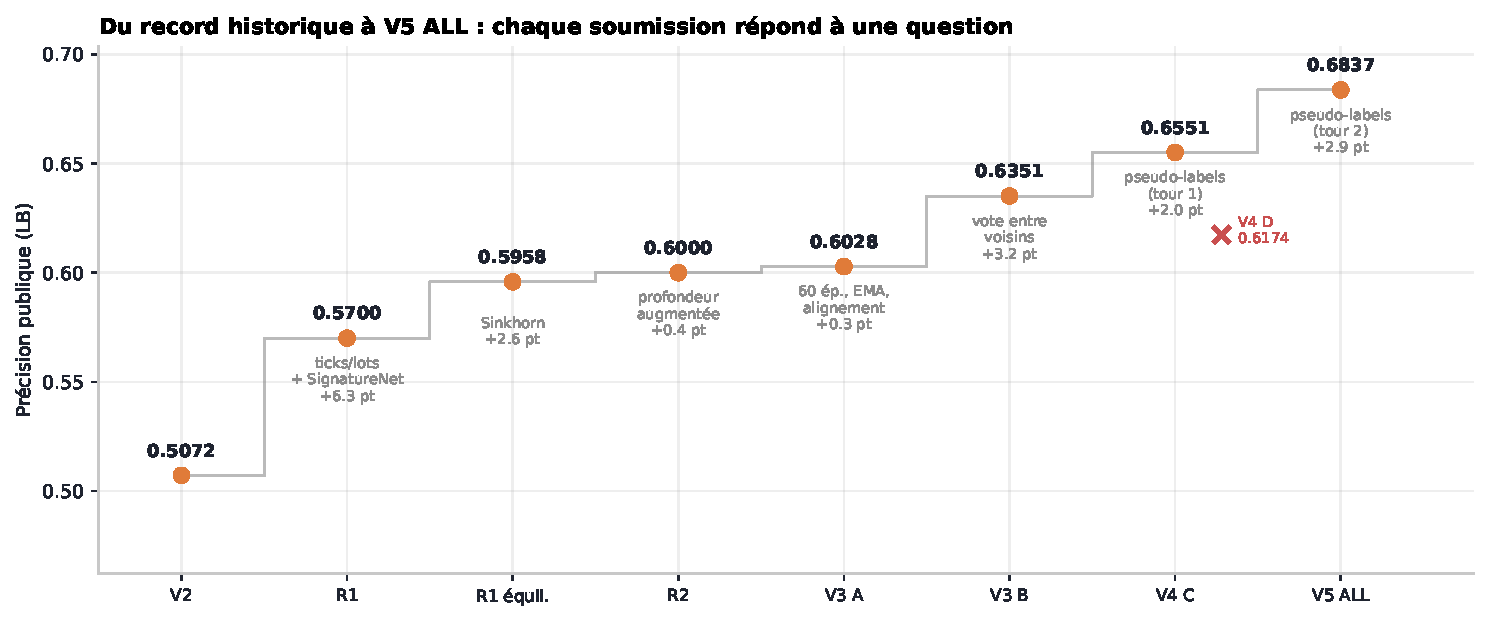
\includegraphics[width=\linewidth]{figures/v5_lb_journey.pdf}
\caption{Accuracy publique, soumission par soumission, avec le levier ajouté à chaque étape. La croix rouge est une soumission de contrôle (V4~D : V4~C sans les élèves). Section~\ref{sec:selftrain} pour V4 et V5.}
\label{fig:lb}
\end{figure}

\subsection{Contributions et honnêteté du propos}
\begin{enumerate}
\item Une couche de données \emph{validée} : alignement par \code{obs\_id}, contiguïté, renumérotation des ordres qui ne conserve que les égalités (section~\ref{sec:donnees}).
\item Une représentation en unités naturelles. Nous montrons formellement ce que la normalisation par médiane locale efface (section~\ref{sec:unites}).
\item Des tokens d'événements sans aucun seuil appris, et des statistiques de parcours d'ordres calculées de façon vectorisée et exacte (section~\ref{sec:ordres}), illustrés sur un exemple complet calculé par le code lui-même (section~\ref{sec:exemple}).
\item Un entonnoir de screening : utilité contre dérive, AUC adversariale, ajout et retrait réentraînés, intervalles appariés (section~\ref{sec:screening}).
\item SignatureNet, décrit équation par équation, avec un décompte exact de ses paramètres (section~\ref{sec:signaturenet}).
\item La correction de prior par Sinkhorn : dérivation, convergence, conditions de validité, effet observé (section~\ref{sec:sinkhorn}).
\item Un atlas de la donnée réelle (section~\ref{sec:atlas}) et une démonstration contrôlée de 25 modèles sur un même protocole, qui isole l'apport de la représentation : +16 points à architecture égale (section~\ref{sec:demo}).
\item L'auto-apprentissage transductif : filtre d'accord entre deux lectures du professeur, quota équilibré par titre, deux tours, soumissions de contrôle et analyse de la contamination des mesures internes (section~\ref{sec:selftrain}).
\end{enumerate}
\noindent Ce que ce document \emph{ne} prétend \emph{pas}. Les $+6{,}3$ points du premier run mêlent représentation, architecture et ensemble : un seul score public ne permet pas de les séparer, et la démonstration de la section~\ref{sec:demo} ne les sépare qu'en interne. Les gains de validation ne sont pas des gains de test. L'équilibrage suppose un test équilibré entre titres et utilise les entrées du test, comme le vote entre voisins et l'auto-apprentissage : leur conformité au règlement est à vérifier. Les mesures internes des élèves V4/V5 sont contaminées par leur professeur : seul le LB y tranche. Enfin, les résultats synthétiques cités en annexe valident le logiciel, jamais la performance.
